\subsection{Temperature Sensor}
\begin{figure}[h!]
	\centering
 	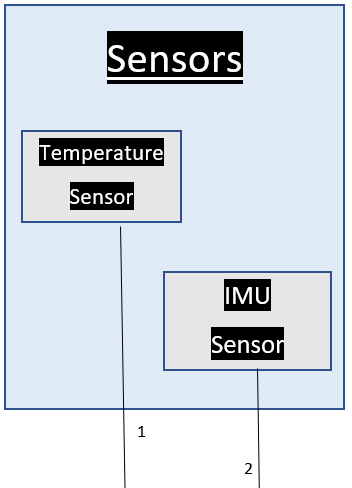
\includegraphics[width=0.60\textwidth]{images/Sensors subsystems}
 \caption{Sensor subsystems description}
\end{figure}

\subsubsection{Assumptions}
Temperature sensors are built in on Arduino Nano 33 BLE sense which can have small error during the temperature read which can be adjusted though Arduino Programming.

\subsubsection{Responsibilities}
Arduino nano built in temperature sensor reads temperature. Arduino software provides HTS221 library to read temperature from Arduino nano 33 BLE sense. HTS221.h handles temperature readings from Arduino nano board and it must be included during Arduino programming.
\newpage
\begin{lstlisting}
#include <Arduino_HTS221.h>		//Arduino library to be included
HTS.begin()				//Initializes temperature sensor 
-	Returns true of false depending on the initialization
HTS.readTemperature()			//Function to read temperature in degree Celsius
        -  Returns temperature in degree Celsius (default)
HTS.readTemperature(FAHRENHEIT)
-	Returns temperature in Fahrenheit if needed
\end{lstlisting}

\subsubsection{Subsystem Interfaces}
Each of the inputs and outputs for the subsystem are defined here. Create a table with an entry for each labelled interface that connects to this subsystem. For each entry, describe any incoming and outgoing data elements will pass through this interface.

\begin {table}[H]
\caption {Subsystem interfaces} 
\begin{center}
    \begin{tabular}{ | p{1cm} | p{6cm} | p{3cm} | p{3cm} |}
    \hline
    ID & Description & Inputs & Outputs \\ \hline
     & Temperature interface & \pbox{3cm}{N/A} & \pbox{3cm}{output 1}  \\ \hline
    \end{tabular}
\end{center}
\end{table}
\newpage

\subsection{IMU Sensor}

\begin{figure}[h!]
	\centering
 	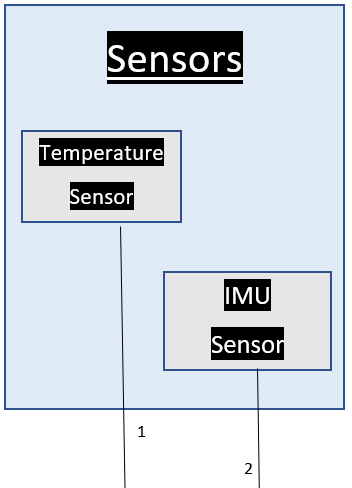
\includegraphics[width=0.60\textwidth]{images/Sensors subsystems}
 \caption{Sensor subsystems description}
\end{figure}

\subsubsection{Assumptions}
Depending on the Bluetooth Hydrometer case, there might me some fluctuation in IMU readings which can be adjusted within the Arduino software.

\subsubsection{Responsibilities}
Arduino nano 33 BLE sense is an advance microcontroller, it consists of 9-axis Inertial Measurement Unit (IMU) which refers to built-in gyroscope, accelerometer and magnetometer. For our project, we will be using gyroscope and accelerometer only. Accelerometer and gyroscope reading are handled by LSM9DS1 library in Arduino. LSM9DS1 library must be included during Arduino nano programming. LSM9DS1 has built-in functions to read from accelerometer and gyroscope.

\begin{lstlisting}
#include <Arduino_LSM9DS1.h>			//Arduino library to be included for IMU
IMU.begin()					//Initialize IMU
-	Returns 1 on success and 0 on failure
\end{lstlisting}

Accelerometer helps to read the device relative orientation on X, Y and Z-axis. It returns values of X, Y and Z based on tilt as shown in figure 5. 

\begin{lstlisting}
IMU.accelerationAvailable()
-	Returns 0 if no new acceleration data is available
-	Returns 1 if new acceleration data is available

IMU.readAcceleration(x, y, z)
-	1 on success and 0 on failure
-	X, y and z are float variables where acceleration values will be stored
\end{lstlisting}

IMU acceleration read step shown below

\begin{lstlisting}
If(IMU.accelerationAvailable()){
		IMU.readAcceleration(x, y, z);
\end{lstlisting}

Gyroscope reads the relative rotation of Arduino board on X, Y and Z-axis. It returns values of X, Y and Z based on angle of rotation of axis, i.e. upside down or upside position. Y-axis value is used for the project to determine the rotation of Arduino nano. X and Z-axis value is not prioritized as Arduino should be floating in upright position while reading values from Arduino (Y-axis matters).
Gyroscope read is same as accelerometer read.

\begin{lstlisting}
IMU.gyroscopeAvailable()
-	Returns 0 if no new gyroscope data sample is available
-	Returns 1 if new gyroscope data sample is available
IMU.readGyroscope(x, y, z)
-	1 on success, 0 on failure
-	X, y, z are float variables where the gyroscope values will be stored
\end{lstlisting}

IMU gyroscope read steps shown below,

\begin{lstlisting}
If(IMU.gyroscopeAvailable()){
		IMU.readGyroscope(x, y, z);
\end{lstlisting}

\begin{figure}[h!]
	\centering
 	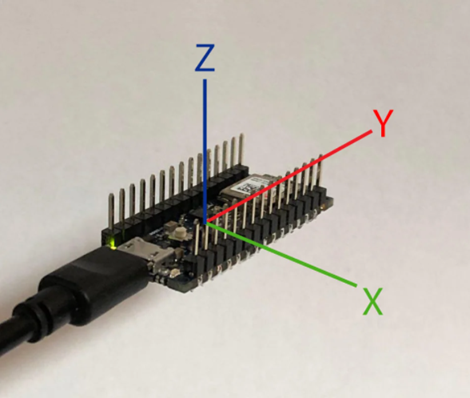
\includegraphics[width=0.60\textwidth]{images/arduino_relative_position}
 \caption{Arduino relative position on X, Y and Z axis's}
\end{figure}

\subsubsection{Subsystem Interfaces}
Each of the inputs and outputs for the subsystem are defined here. Create a table with an entry for each labelled interface that connects to this subsystem. For each entry, describe any incoming and outgoing data elements will pass through this interface.

\begin {table}[H]
\caption {Subsystem interfaces} 
\begin{center}
    \begin{tabular}{ | p{1cm} | p{6cm} | p{3cm} | p{3cm} |}
    \hline
    ID & Description & Inputs & Outputs \\ \hline
     & IMU interface & \pbox{3cm}{N/A} & \pbox{3cm}{output 2}  \\ \hline
    \end{tabular}
\end{center}
\end{table}


